% !TeX root = RJwrapper.tex
\title{Puremoe: A PMID-Centered R Interface to PubMed and NIH/NLM Literature Data}


\author{by Jason Timm}

\maketitle

\abstract{%
Biomedical literature projects commonly begin in PubMed but require data from several additional National Institutes of Health and National Library of Medicine services. These services differ in their interfaces, response formats, batching rules, and data structures. The puremoe package provides a PMID-centered R interface for searching PubMed and retrieving article metadata, iCite metrics and citation links, PubTator3 annotations and relations, and open-access PubMed Central full text. It keeps remote retrieval explicit and provides source-specific local workflows for MeSH keyness, citation snowballing and network construction, and sentence-level context for biomedical entities and relations. We describe the package's design, compare its scope with adjacent R clients, and demonstrate the workflow with a dated corpus on buprenorphine and opioid use disorder. puremoe is intended for moderately sized literature projects that require a structured NIH/NLM-centered corpus without maintaining separate API clients or a local literature index.
}

\section{Introduction}\label{introduction}

PubMed is the principal public gateway to the biomedical journal literature,
but searching it is only one part of many literature-analysis workflows
\citep{lu2011pubmed}. PubMed records provide bibliographic metadata and Medical
Subject Headings (MeSH), the controlled vocabulary used to index MEDLINE
\citep{lipscomb2000mesh}. Complementary NIH and NLM services add other forms of
evidence: iCite supplies article-level citation measures and citation links
\citep{hutchins2016rcr}, PubTator3 identifies biomedical entities and relations in
text \citep{wei2024pubtator}, and PubMed Central (PMC) distributes open-access full
text. PMIDs connect these resources conceptually, yet the resources do not
share a single programming interface.

The resulting integration work is substantial even when the scientific
question is modest. Each service has distinct request conventions, batch sizes,
rate limits, response formats, and data models. An R workflow may therefore need
to divide the same PMID vector several ways, parse XML, JSON, and BioC data, and
preserve nested annotations without duplicating articles. Combining citation
data, controlled vocabulary, and biomedical annotations requires both reliable
retrieval and representations that remain usable after retrieval.

\texttt{puremoe} \citep{timm2026puremoe} treats this task as a PMID-centered integration
problem. Its contribution is not a new literature database or search language.
It turns a PubMed-derived or user-supplied PMID set into reusable R objects that
can be enriched across selected NIH/NLM services and passed into local workflows
without hidden retrieval. A compact interface covers PubMed, iCite, PubTator3,
and PMC \citep{roberts2001pmc};
the corresponding local workflows include MeSH keyness, citation-neighborhood
expansion and network construction, and sentence-level context for biomedical
entities and relations. Keeping retrieval and local computation separate makes
the intermediate objects available for inspection, saving, joining, or analysis
with ordinary R tools.

The package also ships a PubMed-wide snapshot of MeSH descriptor frequencies,
which supplies the background distribution needed to distinguish descriptors
that characterize a selected corpus from headings that are merely common
throughout PubMed.

This article positions \texttt{puremoe} among adjacent R clients, describes its
interface and data model, and demonstrates the workflow with a corpus on
buprenorphine and opioid use disorder. The final sections discuss
implementation, performance, reproducibility, and
the limits of the package's deliberately NIH/NLM-centered scope.

\section{Existing approaches in R}\label{existing-approaches-in-r}

R already has capable clients for several parts of this workflow. \texttt{rentrez}
provides a general interface to NCBI E-utilities and supports the
many databases in the Entrez system \citep{winter2017rentrez}. \texttt{easyPubMed}
\citep{fantini2025easypubmed} and \texttt{pubmedR} \citep{aria2026pubmedr} focus more directly on
PubMed retrieval and parsing; \texttt{pubmedR} also provides citation-oriented helpers
and data that can enter a \texttt{bibliometrix} workflow. These packages are natural
choices when PubMed records, rather than coordinated access to several NIH/NLM
services, are the primary object of interest.

Two broader scholarly-data clients provide important points of comparison.
\texttt{europepmc} \citep{jahn2023europepmc} exposes the Europe PMC search index, references
and citing works, annotations, and available full text; the underlying service
integrates records from multiple life-science sources \citep{ferguson2021europepmc}.
\texttt{openalexR} targets the cross-disciplinary OpenAlex scholarly graph and includes
operations for retrieving citation neighborhoods \citep{aria2024openalexr}. Their
broader indexes can be preferable to a PubMed-centered workflow when source
breadth or cross-domain citation analysis is the main requirement.

The overlap among these packages does not make their operations equivalent.
Europe PMC annotations are not identical to direct PubTator3 output, an
OpenAlex open-access location is not parsed PMC XML, and generic access to an
Entrez endpoint does not by itself provide a MeSH keyness calculation or an
evidence-bearing entity relation network. Table 1 therefore records operations
exposed as native package workflows. ``Generic'' denotes a task that can be
constructed through a lower-level interface, rather than a dedicated operation
with the same returned structure.

\begin{table*}
\centering
\caption{\label{tab:package-comparison}Native, documented capabilities in puremoe and adjacent R packages. Documentation was audited for puremoe 1.1.1, rentrez 1.2.4, easyPubMed 3.1.6, pubmedR 1.0.2, europepmc 0.4.3, and openalexR 3.1.0.}
\centering
\resizebox{\ifdim\width>\linewidth\linewidth\else\width\fi}{!}{
\fontsize{6.5}{8.5}\selectfont
\begin{tabular}[t]{l|c|c|c|c|c|c}
\hline
capability & puremoe & rentrez & easyPubMed & pubmedR & europepmc & openalexR\\
\hline
Direct PubMed/NCBI search & Native & Native & Native & Native & Partial & —\\
\hline
PubMed abstracts and metadata & Native & Generic / partial & Native & Native & Native & Partial\\
\hline
Retrieve an existing PMID set & Native & Native & Native & Native & Native & Partial\\
\hline
NIH iCite metrics and links & Native & — & — & — & — & —\\
\hline
PubTator3 entities and relations & Native & — & — & — & Partial & —\\
\hline
PMC open-access full text & Native & Generic / partial & — & — & Native & Partial\\
\hline
MeSH terms in article records & Native & Generic / partial & Native & Native & Native & —\\
\hline
MeSH thesaurus and tree data & Native & Generic / partial & — & — & — & —\\
\hline
References and citing works & Native & Generic / partial & Partial & Native & Native & Native\\
\hline
Citation snowballing helper & Native & — & — & — & — & Native\\
\hline
Ready-to-use citation network & Native & — & — & — & — & Partial\\
\hline
MeSH corpus keyness & Native & — & — & — & — & —\\
\hline
Sentence-level entity context and evidence network & Native & — & — & — & — & —\\
\hline
\end{tabular}}
\end{table*}

Several qualifications are important when reading Table 1. \texttt{europepmc}
searches the Europe PMC index, which includes MEDLINE records, rather than
sending a query to NCBI PubMed. Its annotations are related text-mining data
but are not a direct PubTator3 client. \texttt{rentrez} can reach PMC, MeSH, and NCBI
link sets through the generic Entrez interface, but users must choose the
databases and link types and then perform the corresponding parsing and
analysis. \texttt{easyPubMed} can extract references present in PubMed XML; this is not
a general cited-by service. Finally, OpenAlex works can carry PMIDs and
open-access locations, but \texttt{openalexR} is neither a PubMed client nor a PMC XML
parser; its snowballing output requires a further step to become a graph.

The comparison is therefore a statement of scope, not a claim that \texttt{puremoe}
replaces these clients. Its narrower contribution is a consistent path through
selected NIH/NLM literature services followed by local workflows designed for
the resulting objects. Broader NCBI or scholarly-graph questions remain better
served by \texttt{rentrez} or \texttt{openalexR}, while Europe PMC-centered work is naturally
handled by \texttt{europepmc}.

\section{Package design}\label{package-design}

Three choices organize the package: PMIDs provide the common key, remote
retrieval is explicit, and one compact dispatcher exposes endpoint-specific
operations. Retrieved objects then enter source-specific local workflows rather
than a general analysis framework.

\subsection{PMIDs as the common key}\label{pmids-as-the-common-key}

PMIDs are the organizing key rather than an incidental field. Users may begin
with \texttt{search\_pubmed()} or supply identifiers collected elsewhere. The same
character vector is then reusable across PubMed, iCite, and PubTator3. PMC is
the one qualified case: PMIDs are first resolved to open-access XML locations.
This organization minimizes identifier reconciliation and makes joins across
returned tables explicit. Figure 1 summarizes the data flow: remote services
enrich a common corpus, normalized objects form the boundary of the retrieval
layer, and local workflows consume those objects.

\begin{figure}

{\centering 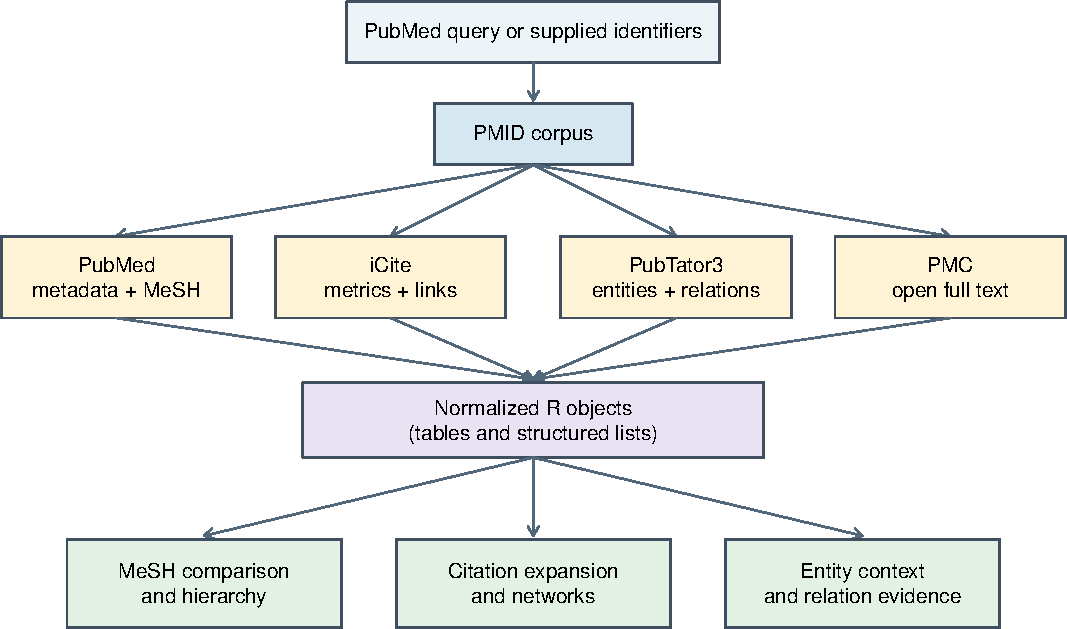
\includegraphics[width=1\linewidth]{timm_files/figure-latex/package-architecture-1} 

}

\caption{PMID-centered package architecture. Solid arrows show retrieval and transformation; the lower row contains local workflows that make no additional service requests.}\label{fig:package-architecture}
\end{figure}

\subsection{Retrieval and local workflows}\label{retrieval-and-local-workflows}

The public retrieval layer consists primarily of \texttt{search\_pubmed()} and
\texttt{get\_records()}. The former resolves a PubMed query to PMIDs; the latter
dispatches a PMID vector or endpoint-specific identifiers to a selected source.
Endpoint-specific batching, requests, and parsing remain behind this shared
surface. The returned tables and lists then enter local workflows designed for
their source structures, without making additional API requests
\citep{timm2026puremoe}.

Each local workflow follows the structure of its source. \texttt{mesh\_keyness()} uses
retrieved PubMed records, \texttt{citation\_network()} uses an iCite result already in
memory, and the PubTator3 context functions use a previously returned
entity/relation object. These functions accept retrieved data and make no
further service requests. They return tables that users can save, filter, join,
or pass to other R tools. Users can therefore revise a threshold, network, or
display without sending new requests to an upstream service.

\subsection{Endpoint schemas}\label{endpoint-schemas}

The supported endpoints differ in both their accepted inputs and returned
objects. Table 2 is generated from \texttt{endpoint\_info()} rather than maintained as
a separate handwritten schema, so it describes the installed package version.

\begin{table*}
\centering
\caption{\label{tab:endpoint-schemas}Remote endpoints exposed by the shared retrieval function.}
\centering
\resizebox{\ifdim\width>\linewidth\linewidth\else\width\fi}{!}{
\fontsize{8}{10}\selectfont
\begin{tabular}[t]{>{\raggedright\arraybackslash}p{2.6cm}|>{\raggedright\arraybackslash}p{3cm}|>{\raggedright\arraybackslash}p{3.4cm}|>{\raggedright\arraybackslash}p{3.6cm}}
\hline
endpoint & source & input & returns\\
\hline
pubmed\_abstracts & PubMed E-utilities & PMIDs & data.table; one row per PMID\\
\hline
pubmed\_affiliations & PubMed E-utilities & PMIDs & data.table; one row per author-affiliation record\\
\hline
icites & NIH iCite & PMIDs & data.table; one row per PMID returned by iCite\\
\hline
pubtator & PubTator3 BioC JSON export & PMIDs & list with entities and relations data.tables\\
\hline
pmc\_fulltext & PMC Cloud Service XML files & HTTPS XML URLs, usually from pmid\_to\_ftp()\$url & data.table; one row per parsed top-level body section\\
\hline
\end{tabular}}
\end{table*}

As Table 2 shows, the \texttt{endpoint} argument keeps the public retrieval surface
small while allowing the implementation to use service-specific request and
parsing strategies.
\texttt{endpoint\_info()} makes those differences inspectable: for each endpoint it
reports the upstream source, accepted input, returned object, relevant
parameters, rate-limit guidance, and endpoint-specific notes. This metadata is
part of the interface rather than a substitute for it; returned objects use
stable package-level column names even though the remote representations differ.

\section{Worked example: Buprenorphine and opioid use disorder}\label{worked-example-buprenorphine-and-opioid-use-disorder}

The example corpus contains PubMed records explicitly centered on
buprenorphine and opioid use disorder (OUD). Requiring both concepts in article
titles supplies a transparent precision rule and keeps the live workflow
manageable. Buprenorphine is well established in maintenance treatment, and
comparisons with methadone and other treatment strategies provide a literature
with chemical, disease, intervention, and outcome concepts
\citep{mattick2014buprenorphine}. The example follows one corpus through a connected
sequence: PubMed defines it, MeSH characterizes it, iCite tests what its title
wording leaves outside, PubTator3 makes predicted relations inspectable in text,
and PMC supplies selected full text for deeper reading. The query does not
define a systematic-review search: in particular, its contemporary title
wording underrepresents older literature described with terms such as \emph{opioid
dependence}.

\subsection{Corpus definition and article metadata}\label{corpus-definition-and-article-metadata}

The workflow first defines a transparent seed set in a reusable form. It begins
with the literal PubMed query; \texttt{search\_pubmed()} returns the PMID vector that
serves as the input to every subsequent enrichment.

\begin{verbatim}
query <- 'buprenorphine[Title] AND "opioid use disorder"[Title]'
pmids <- puremoe::search_pubmed(query)
\end{verbatim}

The query returned 784 identifiers on
2026-09-11. Recording both the literal query and
date is necessary because PubMed is a changing index. The example intentionally
favors a transparent selection rule over maximal recall; later citation
expansion provides an empirical view of what this narrow wording leaves outside
the seed set.

The seed PMIDs are passed to the shared retrieval function with the PubMed
metadata endpoint. The parallelism and delay are explicit retrieval parameters,
not global package state. Table 3 shows five returned records and the principal
article-level fields used later in the workflow.

\begin{verbatim}
abstracts <- puremoe::get_records(
  pmids,
  endpoint = "pubmed_abstracts",
  cores = 3L,
  sleep = 1.05
)
\end{verbatim}

\begin{table*}[!h]
\centering
\caption{\label{tab:abstract-preview}Example PubMed records returned by the shared retrieval function.}
\centering
\resizebox{\ifdim\width>\linewidth\linewidth\else\width\fi}{!}{
\fontsize{8}{10}\selectfont
\begin{tabular}[t]{>{\raggedright\arraybackslash}p{1.4cm}|>{\raggedleft\arraybackslash}p{0.8cm}|>{\raggedright\arraybackslash}p{3.4cm}|>{\raggedright\arraybackslash}p{7cm}}
\hline
pmid & year & journal & articletitle\\
\hline
42709580 & 2026 & Journal of addiction medicine & Treatment Discontinuation and Barriers and Facilitators to Retention Among Individuals Initiating Buprenorphine for Opioid Use Disorder: A Longitudinal Cohort Study.\\
\hline
42644692 & 2026 & The American journal of drug and alcohol abuse & Extended-release naltrexone versus buprenorphine-naloxone for opioid use disorder: a systematic review and meta-analysis of randomized controlled trials.\\
\hline
42642688 & 2026 & AIDS and behavior & Trends in Buprenorphine Prescribing Among Adults with Opioid Use Disorder and Coexisting HIV or Viral Hepatitis, 2015-2025.\\
\hline
42613192 & 2026 & Substance use \& addiction journal & Toward a Pharmacy-Led Value-Based Care Model for Buprenorphine Initiation and Management (PharmValue): Development of a Scalable Pharmacist-Led Collaborative Practice Agreement for Medications for Opioid Use Disorder.\\
\hline
42607586 & 2026 & Drug and alcohol dependence & Predictors of incident anxiety and stress-related diagnoses following buprenorphine initiation among commercially insured patients with opioid use disorder.\\
\hline
\end{tabular}}
\end{table*}

In Table 3, each returned article occupies one row, while
nested annotations such as MeSH descriptors are retained in list-columns rather
than flattened into duplicated article rows. This representation preserves an
article-level unit for joins and is also the input subsequently consumed by
\texttt{mesh\_keyness()}.

The same seeds can acquire complementary evidence without identifier
reconciliation. Changing only \texttt{endpoint} enriches them with citation and
biomedical text-mining data. Keeping both calls together emphasizes the common
retrieval pattern and the reuse of one identifier vector.

\begin{verbatim}
icites <- puremoe::get_records(
  pmids,
  endpoint = "icites",
  cores = 3L,
  sleep = 0.25
)
pubtator <- puremoe::get_records(
  pmids,
  endpoint = "pubtator",
  cores = 3L,
  sleep = 0.34
)
\end{verbatim}

The iCite result retains one row per seed returned by the upstream service,
with metrics and citation links in article-level fields and list-columns; it
becomes the input to both expansion and within-corpus network construction. In
the reported snapshot, PubMed returned records for
779 and iCite for
778 of the 784 requested PMIDs; corpus
percentages below use the returned PubMed records. The absent identifiers are
recorded in the retrieval audit supplied with the article; \texttt{get\_records()} binds the
records supplied by the endpoint rather than manufacturing placeholder rows.
PubTator3 instead returns BioC JSON in
which passages contain nested entity annotations and a separate document-level
list contains typed relation assertions. \texttt{get\_records()} parses that structure
into two PMID-linked tables: one row per entity mention and one row per predicted
relation. Entity rows preserve labels, identifiers, offsets, and source
passages, while relation rows identify their endpoints through mention indices.
Sentence context is added locally later in the workflow.

\subsection{MeSH descriptors and corpus keyness}\label{mesh-descriptors-and-corpus-keyness}

MeSH characterizes the seeds in controlled-vocabulary terms that extend beyond
the words used in their titles. The workflow first inspects the vocabulary
attached to individual records and then compares its corpus prevalence with a
PubMed-wide reference. \texttt{puremoe} supplies the vocabulary, hierarchy, and
frequency resources needed for both steps as local R objects.

\texttt{puremoe} exposes the MeSH vocabulary and its tree placements as two tabular
resources. The first supports term-to-descriptor lookup; the second preserves
the potentially multiple hierarchical locations of each descriptor. Tables 4
and 5 show these two representations for the concepts defining the example.

\begin{verbatim}
mesh_thesaurus <- puremoe::data_mesh_thesaurus()
mesh_trees <- puremoe::data_mesh_trees()
\end{verbatim}

\begin{table*}[!h]
\centering
\caption{\label{tab:mesh-term-table}MeSH descriptors and example entry terms.}
\centering
\resizebox{\ifdim\width>\linewidth\linewidth\else\width\fi}{!}{
\fontsize{8}{10}\selectfont
\begin{tabular}[t]{>{\raggedright\arraybackslash}p{3cm}|>{\raggedright\arraybackslash}p{1.8cm}|>{\raggedright\arraybackslash}p{7.8cm}}
\hline
DescriptorName & DescriptorUI & entry\_terms\\
\hline
Buprenorphine & D002047 & Buprenorphine; Subutex; Temgésic; Buprex; Temgesic; Buprenorphine Hydrochloride\\
\hline
Opioid-Related Disorders & D009293 & Opioid-Related Disorders; Opioid-Related Disorder; Opioid Related Disorders; Addiction, Opioid; Dependence, Opioid; Opiate Addiction\\
\hline
\end{tabular}}
\end{table*}

\begin{table*}
\centering
\caption{\label{tab:mesh-tree-table}Hierarchical locations of the example descriptors.}
\centering
\resizebox{\ifdim\width>\linewidth\linewidth\else\width\fi}{!}{
\fontsize{8}{10}\selectfont
\begin{tabular}[t]{>{\raggedright\arraybackslash}p{1.4cm}|>{\raggedright\arraybackslash}p{2.6cm}|>{\raggedright\arraybackslash}p{2.6cm}|>{\raggedright\arraybackslash}p{2.6cm}|>{\raggedright\arraybackslash}p{3.4cm}}
\hline
DescriptorUI & DescriptorName & tree\_location & category & branch\\
\hline
D002047 & Buprenorphine & D03.132.577.249.150 & Chemicals and Drugs & Alkaloids\\
\hline
D002047 & Buprenorphine & D03.605.497.150 & Chemicals and Drugs & Heterocyclic Compounds, Bridged-Ring\\
\hline
D002047 & Buprenorphine & D03.633.400.686.150 & Chemicals and Drugs & Heterocyclic Compounds, Fused-Ring\\
\hline
D002047 & Buprenorphine & D04.615.723.795.150 & Chemicals and Drugs & Polycyclic Aromatic Hydrocarbons\\
\hline
D009293 & Opioid-Related Disorders & C25.775.643.500 & Diseases & Substance-Related Disorders\\
\hline
D009293 & Opioid-Related Disorders & F03.900.647.500 & Psychiatry and Psychology & Substance-Related Disorders\\
\hline
\end{tabular}}
\end{table*}

Table 4 connects preferred descriptors to entry terms and supplementary
concepts. In this example, \emph{Dependence, Opioid} appears as an entry term for
\emph{Opioid-Related Disorders}, making a terminological bridge that the literal
title query does not provide. Table 5 represents hierarchical placement
separately: buprenorphine occupies several chemical branches, while
opioid-related disorders appears under both disease and psychiatry/psychology
branches. A single descriptor-to-parent column would lose that multiplicity.
Keeping both resources as ordinary tables permits direct lookup, joining, and
aggregation with other R tools.

\texttt{mesh\_keyness()} compares the proportion of corpus articles indexed with each
descriptor against its prevalence across PubMed. By default, it uses the
package's bundled \texttt{data\_mesh\_frequencies} snapshot, making the comparison a
local operation. In the package version used for this article, that baseline
was constructed in April 2026
from 39,703,112 distinct PMIDs in a local PubMed mirror; descriptor metadata
came from the contemporaneous NLM MeSH thesaurus. Users may supply another
frequency table when appropriate.

The baseline distinguishes descriptors characteristic of the corpus from broad
headings that are frequent throughout PubMed, while \texttt{min\_count} excludes very
rare corpus descriptors from the ranking.

\begin{verbatim}
keyness <- puremoe::mesh_keyness(
  abstracts,
  measure = "log_odds",
  min_count = 5L
)
\end{verbatim}

The most frequent MeSH descriptors in this archived corpus were
\emph{Humans} (626), \emph{Opioid-Related Disorders} (623), \emph{Buprenorphine} (589), \emph{Opiate Substitution Treatment} (434), \emph{Female} (322), and \emph{Adult} (302). Frequency alone therefore mixes descriptors central to
the topic with broad indexing categories. Table 6 instead reports the six
descriptors ranked highest by standardized log odds, together with the keyness
values and the prevalences being contrasted.

\begin{table*}
\centering
\caption{\label{tab:mesh-keyness-table}MeSH descriptors ranked highest by standardized log odds against the PubMed-wide baseline.}
\centering
\resizebox{\ifdim\width>\linewidth\linewidth\else\width\fi}{!}{
\fontsize{7}{9}\selectfont
\begin{tabular}[t]{l|r|r|r|r|r}
\hline
Descriptor & Corpus articles & Corpus (\%) & PubMed (\%) & Log odds & Standardized z\\
\hline
Opiate Substitution Treatment & 434 & 55.7 & 0.01 & 9.08 & 123.80\\
\hline
Buprenorphine & 589 & 75.6 & 0.02 & 9.61 & 114.33\\
\hline
Narcotic Antagonists & 292 & 37.5 & 0.04 & 7.28 & 97.83\\
\hline
Opioid-Related Disorders & 623 & 80.0 & 0.06 & 8.74 & 97.55\\
\hline
Buprenorphine, Naloxone Drug Combination & 107 & 13.7 & 0.00 & 9.20 & 82.62\\
\hline
Analgesics, Opioid & 294 & 37.7 & 0.17 & 5.87 & 79.36\\
\hline
\end{tabular}}
\end{table*}

Table 6 elevates treatment-specific descriptors that are unusually concentrated
in the corpus rather than simply common in biomedical indexing. The contrast
shows how controlled-vocabulary enrichment can characterize a corpus beyond
words in titles. The scores are descriptive rankings, not independent
hypothesis tests or evidence about comparative treatment effectiveness.

\subsection{Citation-based corpus exploration}\label{citation-based-corpus-exploration}

Citation data expose connected literature omitted by the deliberately narrow
title wording and show how its addition changes the corpus. The iCite result
already in memory supports two local views: an auditable expansion beyond the
seeds and a graph of citations within them.

Following references and citing articles is a well-established complement to
database searching, especially when terminology changes or evidence crosses
indexing boundaries \citep{greenhalgh2005snowballing}. Here, candidates must have at
least two links to the seed neighborhood, and the total returned set is capped
at 2,000 records.

\begin{verbatim}
snowball <- puremoe::citation_snowball(
  icites,
  direction = "both",
  min_links = 2L,
  max_nodes = 2000L
)
\end{verbatim}

The configured threshold produced 778 seeds and
1222 candidates, filling the 2,000-record cap. The cap is a
computational and screening decision, not a claim that the neighborhood is
exhausted. Separate cited and citing counts expose why each candidate was
admitted and allow alternative thresholds without another iCite request.

Candidate PMIDs can be sent back through the same PubMed metadata endpoint.
Table 7 joins those records to their admission counts and lists the strongest
links to the seed neighborhood. The ordinary joins, sorting, and display code
are hidden because they are not additional \texttt{puremoe} operations.

\begin{table*}[!h]
\centering
\caption{\label{tab:expansion-metadata-table}Highest-ranked articles discovered through citation links.}
\centering
\resizebox{\ifdim\width>\linewidth\linewidth\else\width\fi}{!}{
\fontsize{8}{10}\selectfont
\begin{tabular}[t]{>{\raggedright\arraybackslash}p{1.4cm}|>{\raggedleft\arraybackslash}p{0.8cm}|>{\raggedright\arraybackslash}p{5.6cm}|r|r|r}
\hline
pmid & year & articletitle & cited\_links & citing\_links & link\_count\\
\hline
28446428 & 2017 & Mortality risk during and after opioid substitution treatment: systematic review and meta-analysis of cohort studies. & 140 & 1 & 141\\
\hline
24500948 & 2014 & Buprenorphine maintenance versus placebo or methadone maintenance for opioid dependence. & 128 & 0 & 128\\
\hline
29913516 & 2018 & Medication for Opioid Use Disorder After Nonfatal Opioid Overdose and Association With Mortality: A Cohort Study. & 104 & 1 & 105\\
\hline
32022884 & 2020 & Comparative Effectiveness of Different Treatment Pathways for Opioid Use Disorder. & 74 & 4 & 78\\
\hline
25919527 & 2015 & Emergency department-initiated buprenorphine/naloxone treatment for opioid dependence: a randomized clinical trial. & 73 & 0 & 73\\
\hline
23961726 & 2014 & Treatment retention among patients randomized to buprenorphine/naloxone compared to methadone in a multi-site trial. & 65 & 0 & 65\\
\hline
12924748 & 2003 & The Clinical Opiate Withdrawal Scale (COWS). & 59 & 0 & 59\\
\hline
29150198 & 2018 & Comparative effectiveness of extended-release naltrexone versus buprenorphine-naloxone for opioid relapse prevention (X:BOT): a multicentre, open-label, randomised controlled trial. & 57 & 2 & 59\\
\hline
32511106 & 2020 & The ASAM National Practice Guideline for the Treatment of Opioid Use Disorder: 2020 Focused Update. & 54 & 1 & 55\\
\hline
30352671 & 2018 & Risk factors for discontinuation of buprenorphine treatment for opioid use disorders in a multi-state sample of Medicaid enrollees. & 49 & 5 & 54\\
\hline
\end{tabular}}
\end{table*}

\begin{figure}

{\centering 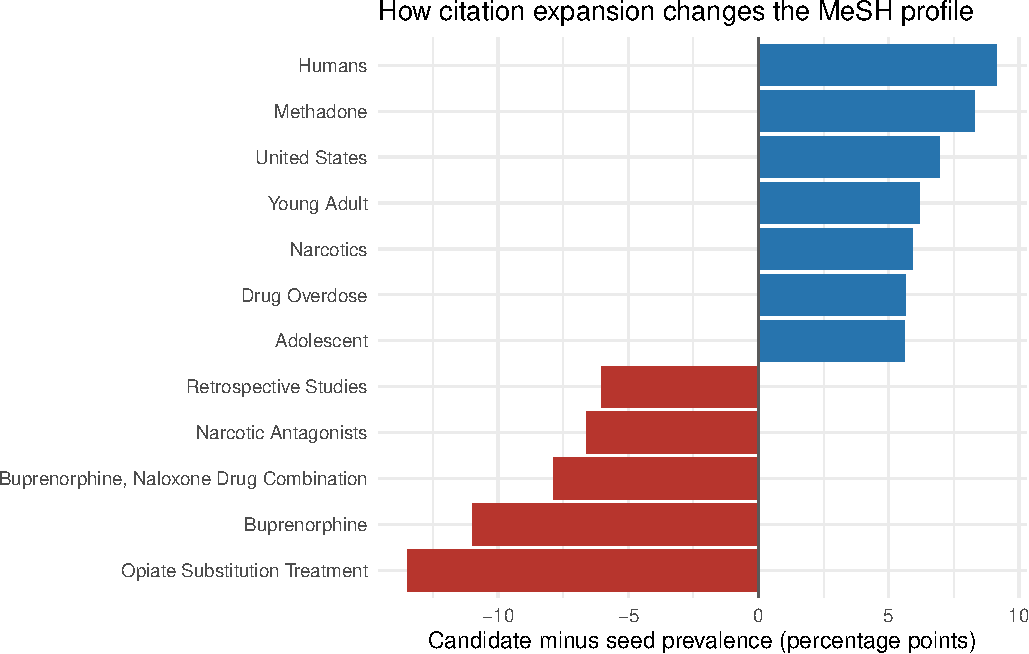
\includegraphics[width=1\linewidth]{timm_files/figure-latex/expansion-mesh-shift-1} 

}

\caption{Difference in MeSH descriptor prevalence between citation-discovered candidates and the title-defined seed corpus. Positive values indicate higher prevalence among candidates; negative values indicate higher prevalence among seeds.}\label{fig:expansion-mesh-shift}
\end{figure}

Table 7 exposes each candidate's admission counts. Several highly connected
records are trials, reviews, and guidelines that predate most seeds; titles
using \emph{opioid dependence} appear prominently. Citation expansion thus
recovers historically connected work that a literal title condition misses.
Figure 2 complements the ranked candidates by comparing MeSH prevalence in the
seeds and the citation-discovered set: positive values identify descriptors
more common among candidates, while negative values identify descriptors
concentrated in the seeds. Neither link rank nor
vocabulary shift establishes relevance on its own, but both provide inspectable
signals for subsequent screening.

The same iCite object can instead be restricted to links within the seed corpus.
\texttt{citation\_network()} returns conventional node and edge tables; one additional
line converts them to an \texttt{igraph} object for standard graph summaries.

\begin{verbatim}
citation_net <- puremoe::citation_network(icites)
citation_graph <- graph_from_data_frame(
  citation_net$edges,
  directed = TRUE,
  vertices = citation_net$nodes
)
\end{verbatim}

The within-corpus graph contains 778 nodes and
1907 directed edges. The presence of
107 isolates and
111 weak components is itself informative: a
topically coherent query need not produce a single connected citation
community. It also cautions against interpreting this graph as complete
scholarly connectivity, because it contains only iCite links among the retained
PubMed records. Returning node and edge tables is more useful than printing an
unlabeled network; users can pass them to \texttt{igraph} \citep{csardi2006igraph} and select
layouts, filters, or network statistics appropriate to the research question.

\subsection{PubTator3 annotations in sentence context}\label{pubtator3-annotations-in-sentence-context}

Citation links test the boundary of the seed corpus; the PubTator3 workflow
returns attention to concepts and predicted relations inside the retrieved
texts. PubTator3 performs biomedical entity and relation extraction and returns
its predictions in BioC structures \citep{wei2024pubtator}. \texttt{get\_records()} flattens
those structures into linked entity mention and relation tables.
\texttt{pubtator\_context()} then performs a lightweight local NLP operation that
attaches sentence context, after which \texttt{pubtator\_cooccurrence()} and
\texttt{pubtator\_network()} construct corpus-level summaries. The package does not
train or run a second biomedical extraction model; its contribution here is
parsing, alignment, aggregation, and retention of the evidence connecting each
summary back to the source PMID and sentence.

\texttt{pubtator\_context()} takes the entity and relation tables returned by
\texttt{get\_records(endpoint\ =\ "pubtator")}. The BioC response contains passage text
and document-relative annotation offsets, so the material needed to reconstruct
context is present, but sentences are not supplied as an analytical table and
are not attached to relation rows. The function groups passages by PMID and
title/abstract location, segments each passage into sentences, and records the
resulting sentence spans. It aligns each entity's document offset with a
sentence span and adds a sentence identifier plus sentence-relative entity
coordinates. It then resolves each relation's two mention indices against the
entity table, adding endpoint text, identifiers, passage locations, and sentence
identifiers. From those fields it derives \texttt{same\_sentence} and
\texttt{sentence\_distance}. The returned \texttt{entities}, \texttt{relations}, and \texttt{sentences}
tables therefore make textual proximity directly queryable without another
service request or a user-written BioC and offset-alignment pipeline.

Once that context exists, \texttt{pubtator\_cooccurrence()} constructs a local summary
from the entity table; it does not use or expand PubTator3's predicted relation
rows. It counts mention pairs within a chosen sentence window. Aggregating
\texttt{by\ =\ "type"} describes broad combinations such as chemical--disease mentions,
whereas \texttt{by\ =\ "entity"} retains the identifiers and mention labels supplied to
the function. The latter makes normalization an explicit composition step: the
article joins PubTator3 identifiers to the MeSH descriptor and supplementary
concept records loaded for Table 4, while preserving the forms attested in the
source text. Identifiers from other vocabularies remain unchanged.

\begin{verbatim}
context <- puremoe::pubtator_context(pubtator)
cooccurrence_types <- puremoe::pubtator_cooccurrence(
  context,
  window = 0L,
  by = "type"
)
\end{verbatim}

\begin{verbatim}
cooccurrence_concepts <- puremoe::pubtator_cooccurrence(
  concept_entities,
  window = 0L,
  by = "entity"
)
\end{verbatim}

\begin{table*}[!h]
\centering
\caption{\label{tab:pubtator-context-table}Most frequent same-sentence entity pairs after MeSH label resolution. Bracketed values are MeSH UIs; attested columns retain source forms.}
\centering
\resizebox{\ifdim\width>\linewidth\linewidth\else\width\fi}{!}{
\fontsize{7}{9}\selectfont
\begin{tabular}[t]{>{\raggedright\arraybackslash}p{1.1cm}|>{\raggedright\arraybackslash}p{2.2cm}|>{\raggedright\arraybackslash}p{1.8cm}|>{\raggedright\arraybackslash}p{1.1cm}|>{\raggedright\arraybackslash}p{2.2cm}|>{\raggedright\arraybackslash}p{1.8cm}|r|r}
\hline
type\_x & concept\_x & attested\_x & type\_y & concept\_y & attested\_y & n & n\_pmids\\
\hline
Chemical & Buprenorphine [D002047] & buprenorphine; Buprenorphine; BUP & Disease & Opioid-Related Disorders [D009293] & OUD; opioid use disorder; Opioid Use Disorder & 1869 & 723\\
\hline
Chemical & Buprenorphine [D002047] & buprenorphine; Buprenorphine; BUP & Species & patients & patients & 716 & 321\\
\hline
Disease & Opioid-Related Disorders [D009293] & OUD; opioid use disorder; Opioid Use Disorder & Species & patients & patients & 523 & 266\\
\hline
Chemical & Buprenorphine [D002047] & buprenorphine; Buprenorphine; BUP & Chemical & Naloxone [D009270] & naloxone; Naloxone; NLX & 476 & 167\\
\hline
Chemical & Buprenorphine [D002047] & buprenorphine; Buprenorphine; BUP & Chemical & Methadone [D008691] & methadone; Methadone; MET & 431 & 130\\
\hline
Chemical & Naloxone [D009270] & naloxone; Naloxone; NLX & Disease & Opioid-Related Disorders [D009293] & OUD; opioid use disorder; Opioid Use Disorder & 259 & 129\\
\hline
Chemical & Methadone [D008691] & methadone; Methadone; MET & Disease & Opioid-Related Disorders [D009293] & OUD; opioid use disorder; Opioid Use Disorder & 228 & 104\\
\hline
Chemical & Buprenorphine [D002047] & buprenorphine; Buprenorphine; BUP & Species & patient & patient & 150 & 106\\
\hline
Chemical & Methadone [D008691] & methadone; Methadone; MET & Chemical & Naloxone [D009270] & naloxone; Naloxone; NLX & 112 & 34\\
\hline
Disease & Opioid-Related Disorders [D009293] & OUD; opioid use disorder; Opioid Use Disorder & Disease & Substance-Related Disorders [D019966] & addiction; use; SUD & 108 & 73\\
\hline
Chemical & Buprenorphine [D002047] & buprenorphine; Buprenorphine; BUP & Chemical & Naltrexone [D009271] & naltrexone; Naltrexone; NTX & 108 & 35\\
\hline
Chemical & Buprenorphine [D002047] & buprenorphine; Buprenorphine; BUP & Disease & Pain [D010146] & pain; Pain; painful serious illness & 97 & 48\\
\hline
\end{tabular}}
\end{table*}

Chemical--disease pairs dominate same-sentence co-occurrence in this corpus,
appearing 5828
times across
734 PMIDs.
For Table 8, forms such as \emph{OUD} and \emph{opioid use disorder} therefore resolve to
the preferred MeSH label \emph{Opioid-Related Disorders} when PubTator3 supplies the
corresponding UI. Replacing the working copy's mention label before pairing
also de-duplicates multiple forms of one mapped concept within a sentence; the
original forms remain visible in \texttt{attested\_x} and \texttt{attested\_y}. Unmapped entity
types retain their PubTator3 labels and identifiers rather than being forced
into MeSH. Because both contextualization and the vocabulary join are local,
users can change the sentence window or inspect unmapped rows without another
PubTator3 call. Co-occurrence should be interpreted as proximity in text, not
as a biomedical association.

Relations are aggregated only after sentence context has been attached.
\texttt{pubtator\_network()} resolves each endpoint to a node keyed by the PubTator3
concept identifier when available, with a type-scoped surface form as the
fallback. Repeated assertions with the same directed endpoints and relation
type collapse into one edge carrying total assertion, distinct-PMID, and
same-sentence support counts. A separate evidence table preserves one row per
original PubTator3 relation, including its PMID, relation identifier, endpoint
distance, and source sentence when both mentions map to that sentence. The
function therefore does not predict new relations; it converts PubTator3's
document-level assertions into graph-ready corpus summaries without discarding
the rows needed to audit them. Table 9 displays evidence rows for relations
whose endpoints were mapped to the same sentence.

\begin{verbatim}
relation_net <- puremoe::pubtator_network(context)
\end{verbatim}

\begin{table*}[!h]
\centering
\caption{\label{tab:pubtator-network-evidence}Sentence-level evidence retained for PubTator3 relations after MeSH label resolution. Mention columns preserve the source text.}
\centering
\resizebox{\ifdim\width>\linewidth\linewidth\else\width\fi}{!}{
\fontsize{7}{9}\selectfont
\begin{tabular}[t]{>{\raggedright\arraybackslash}p{1.8cm}|>{\raggedright\arraybackslash}p{1.7cm}|>{\raggedright\arraybackslash}p{1.8cm}|>{\raggedright\arraybackslash}p{1.7cm}|>{\raggedright\arraybackslash}p{1.3cm}|>{\raggedright\arraybackslash}p{1cm}|>{\raggedright\arraybackslash}p{3.2cm}}
\hline
from\_concept & from\_mention & to\_concept & to\_mention & relation\_type & pmid & sentence\\
\hline
Buprenorphine [D002047] & BUP & Opioid-Related Disorders [D009293] & OUD & negative correlation & 41063335 & CONCLUSIONS: Overall, the 8-hour intravenous 1200 mcg BUP micro-infusion protocol was well-tolerated...\\
\hline
Buprenorphine [D002047] & buprenorphine & Opioid-Related Disorders [D009293] & OUD & negative correlation & 41100863 & Our data provide early evidence for safety, adherence, and reduced substance use among perinatal pat...\\
\hline
Buprenorphine [D002047] & Buprenorphine & Opioid-Related Disorders [D009293] & Opioid Use Disorder & negative correlation & 41137494 & Trends in Initiation of Buprenorphine for Opioid Use Disorder Among Older Adults....\\
\hline
Naloxone [D009270] & Naloxone & Multiple Sclerosis [D009103] & Multiple Sclerosis & negative correlation & 41143697 & Secondary Trigeminal Neuralgia Due to Multiple Sclerosis in a Patient With Opioid Use Disorder Treat...\\
\hline
Naloxone [D009270] & Naloxone & Trigeminal Neuralgia [D014277] & Trigeminal Neuralgia & positive correlation & 41143697 & Secondary Trigeminal Neuralgia Due to Multiple Sclerosis in a Patient With Opioid Use Disorder Treat...\\
\hline
Naloxone [D009270] & Naloxone & Opioid-Related Disorders [D009293] & Opioid Use Disorder & negative correlation & 41143697 & Secondary Trigeminal Neuralgia Due to Multiple Sclerosis in a Patient With Opioid Use Disorder Treat...\\
\hline
Buprenorphine [D002047] & Buprenorphine & Multiple Sclerosis [D009103] & Multiple Sclerosis & negative correlation & 41143697 & Secondary Trigeminal Neuralgia Due to Multiple Sclerosis in a Patient With Opioid Use Disorder Treat...\\
\hline
Buprenorphine [D002047] & Buprenorphine & Trigeminal Neuralgia [D014277] & Trigeminal Neuralgia & negative correlation & 41143697 & Secondary Trigeminal Neuralgia Due to Multiple Sclerosis in a Patient With Opioid Use Disorder Treat...\\
\hline
\end{tabular}}
\end{table*}

The resulting network has 535 normalized entities and
530 edges supported by
2187 article-level evidence rows. Evidence is kept
separate from aggregated edges so that a summary remains traceable to its
relation label, PMID, mentions, and available sentence anchor. The article-level
join changes display labels, not relation assertions: a valid MeSH UI receives
its preferred thesaurus name, while the adjacent mention column records what
PubTator3 actually linked in the article. Table 9 therefore also shows why this
design matters. Some rows place clinically relevant concepts in an informative
sentence, whereas others expose a relation label unsupported by the sentence
or text misclassified as an entity. PubTator3 relations are model outputs
\citep{wei2024pubtator}, not validated causal claims; the evidence table makes review
and filtering possible before a network is used substantively.

Figure 3 turns the evidence-preserving output into a deliberately focused
display. It retains only same-sentence relations supported by at least two
distinct PMIDs, excludes Species entities, and shows the one-hop neighborhoods
of buprenorphine and OUD together with supported relations among their
neighbors. Selection is based on article support rather than quotas for
relation classes. Direction remains available in the underlying edge table,
but arrowheads are suppressed because several displayed relation types are not
naturally interpreted as directional claims.

\begin{figure}

{\centering 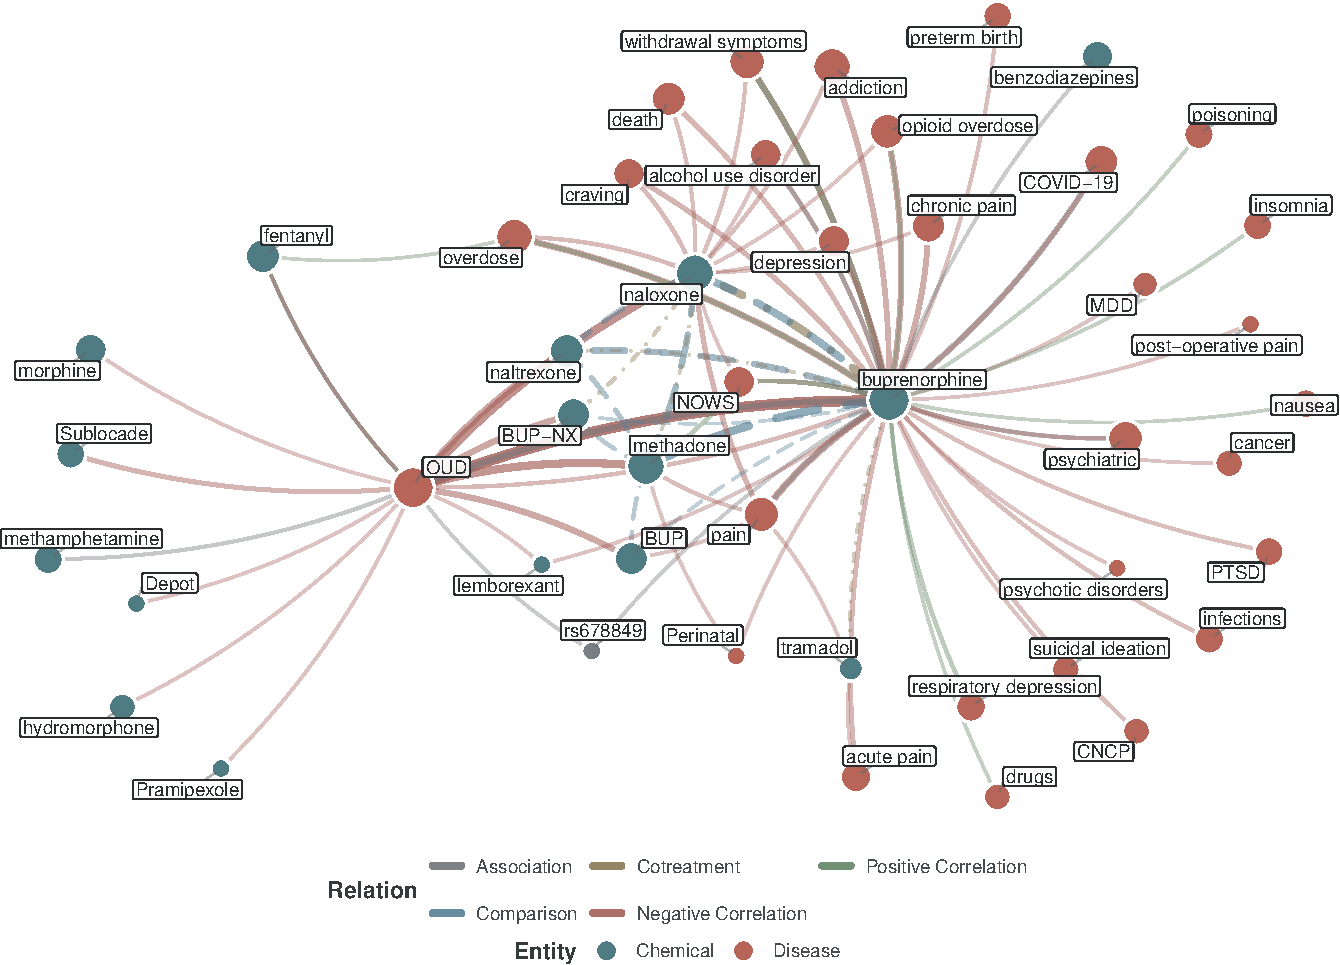
\includegraphics[width=1\linewidth]{timm_files/figure-latex/pubtator-focal-network-1} 

}

\caption{Supported PubTator3 relation neighborhood around buprenorphine and opioid use disorder (OUD). Nodes are entities and colors distinguish entity types; node size increases with the number of supporting PMIDs. Node labels are the most frequent PubTator3 surface form for each concept, whereas Tables 8 and 9 use MeSH preferred names. Edges are same-sentence PubTator3 relations supported by at least two distinct PMIDs; color and line type distinguish relation classes, and width increases with article support. Species entities are excluded. The display summarizes upstream model predictions and should not be interpreted as a validated biomedical or causal network.}\label{fig:pubtator-focal-network}
\end{figure}

The focal display makes the value of the returned graph structure visible:
strongly supported links remain prominent, relation classes retain their
observed frequency, and every edge can still be traced to the evidence rows
used for Table 9. The figure is a downstream view of \texttt{pubtator\_network()}
output, not an additional extraction or graph-inference method.

\subsection{Selective PMC full-text retrieval}\label{selective-pmc-full-text-retrieval}

The example ends with selected source documents. When abstract metadata and
annotations are insufficient, seed PMIDs can be resolved to section-level full
text. This optional step begins by resolving PMIDs to PMC open-data XML
locations. Here, only the first 20 seed PMIDs are passed to the resolver and no
more than three resolved articles are downloaded.

\begin{verbatim}
pmc_probe_pmids <- head(pmids, 20L)
pmc_map <- puremoe::pmid_to_ftp(pmc_probe_pmids, verbose = FALSE)
\end{verbatim}

\texttt{pmid\_to\_ftp()} retains its original function name but, in the package version
used here,
converts eligible PMIDs to versioned XML URLs in PMC's public S3 cloud
distribution rather than the retiring FTP/OA API \citep{nlm2026pmccloud}. The
resolved URLs can then enter the same \texttt{get\_records()} interface used elsewhere
in the article. Table 10 shows the section-level text returned for the selected
articles.

\begin{verbatim}
fulltext_urls <- head(pmc_map$url, 3L)
fulltext <- puremoe::get_records(
  fulltext_urls,
  endpoint = "pmc_fulltext",
  cores = 1L
)
\end{verbatim}

\begin{table*}[!h]
\centering
\caption{\label{tab:pmc-fulltext-table}Representative section text from each retrieved PMC article.}
\centering
\resizebox{\ifdim\width>\linewidth\linewidth\else\width\fi}{!}{
\fontsize{8}{10}\selectfont
\begin{tabular}[t]{>{\raggedright\arraybackslash}p{1.4cm}|>{\raggedright\arraybackslash}p{1.8cm}|>{\raggedright\arraybackslash}p{9.4cm}}
\hline
pmid & section & text\\
\hline
42292651 & Introduction & The opioid epidemic in the United States has been a significant public health issue [1]. In 2020, an estimated 2.5 million U.S. adults had opioid use disorder (OUD) [2], a chronic …\\
\hline
42313747 & Introduction & Chronic pain is commonly reported among people who use drugs (PWUD) [1], with approximately 48\%–60\% of people using prescription opioids non‐medically, compared to 11\%–19\% among th…\\
\hline
42376697 & Introduction & Opioid agonist medications buprenorphine and methadone are the most effective treatments for opioid use disorder (OUD), reducing overdose and HIV‐risk behaviours and improving func…\\
\hline
\end{tabular}}
\end{table*}

Three files are sufficient to demonstrate that \texttt{pmc\_fulltext} converts article
XML into section-level text; this limit is pedagogical rather than an endpoint
restriction. Table 10 normalizes whitespace and shortens displayed values.
Section headings are returned separately in \texttt{section}; for display, a leading
numeric or section label preserved in some source XML is removed when present.
The complete returned \texttt{text} remains unchanged in \texttt{fulltext} for downstream
use. No further text analysis is shown because this example is limited to
section-level retrieval.

\section{Implementation and performance}\label{implementation-and-performance}

The implementation uses endpoint-specific adapters, source-specific local
workflows, and conventional R data structures.

\subsection{Endpoint adapters and execution}\label{endpoint-adapters-and-execution}

\texttt{get\_records()} is a dispatcher over endpoint adapters rather than a common
HTTP request with different URLs. In the package version used here, PubMed and
iCite requests
are divided into batches of at most 199 identifiers, PubTator3 requests into 99,
and PMC full-text requests into five documents. Each adapter constructs the
request expected by its service, parses the response, and returns a stable
package-level representation. PubMed XML becomes an article table with nested
fields; iCite JSON becomes an article table with citation-link list-columns;
PubTator3 BioC data become related entity and relation tables; and PMC's
JATS-formatted XML from the public cloud distribution becomes section-level
text \citep{nlm2026pmccloud}. BioC was created specifically to support portable
biomedical text and annotation exchange \citep{comeau2013bioc}, but its document,
passage, annotation, and relation hierarchy still requires an R representation
suited to downstream analysis.

Independent batches can be evaluated on a user-selected number of parallel
workers. The \texttt{sleep} argument remains exposed because parallel execution does
not waive an upstream service's request policy. The delay is applied within
each worker, so an approximate aggregate ceiling is \texttt{cores\ /\ sleep} requests
per second; callers must choose both values together. The PubMed calls above
use three workers and a 1.05-second delay to remain below NCBI's documented
three-request-per-second limit even without a key. The iCite and PubTator3 calls
used three workers with delays of 0.25 and 0.34 seconds, approximate aggregate
ceilings of 12 and 9 requests per second; users should check each service's
current guidance when choosing these values. NCBI API keys are passed through
where applicable, and an iCite-specific timeout can be set by argument or
package option. These controls are kept at the retrieval boundary; local
functions do not need cores, credentials, sleeps, or retry settings.
\texttt{endpoint\_info()} records these endpoint differences alongside the input and
return schemas so that the compact dispatcher does not conceal
service-specific behavior.

\subsection{Inspectable local workflows}\label{inspectable-local-workflows}

The local workflows remove recurring source-specific wrangling without
attempting to supply a general literature-analysis framework. Their functions
take explicit retrieved objects as inputs, return tables rather than hidden
state, and preserve enough source detail to trace a summary back to the records
that produced it. The three workflow families apply that contract to different
source structures.

\texttt{mesh\_keyness()} compares corpora at the article level, not by counting repeated
labels. It contrasts article-level descriptor prevalence with a PubMed-wide
frequency baseline. The worked example ranks descriptors with a smoothed,
standardized log-odds score. Positive values identify descriptors that are
unusually prevalent in the selected corpus. These descriptive scores depend on
the corpus and baseline version.

The two citation functions retain different links. \texttt{citation\_snowball()} ranks
records outside the seeds by their cited and citing links to the seed
neighborhood. It then applies the requested direction, threshold, and
\texttt{max\_nodes} limit. \texttt{citation\_network()} keeps only links whose endpoints occur
inside the retrieved corpus. Both return the links underlying their summaries.
Users can thus inspect admissions, change thresholds, or construct a graph
without retrieving iCite data again.
Edges follow citation flow: \texttt{from} is the citing PMID and \texttt{to} is the cited
PMID. Accordingly, \texttt{cited\_links} counts seed-to-reference edges and
\texttt{citing\_links} counts candidate-to-seed edges; \texttt{link\_count} is the selected
directional count or their sum. Network nodes are the PMIDs returned by iCite,
including isolates, while edges are deduplicated links whose two endpoints both
belong to that node set.

\texttt{pubtator\_context()} restores textual context to upstream PubTator3 predictions.
The sentence and offset alignment described in the worked example supports two
outputs: co-occurrence summaries calculated from mapped entities and relation
networks that aggregate PubTator3 predictions. The relation networks retain
separate article- and sentence-level evidence rows. These rows allow users to
review useful annotations and extraction errors before substantive
interpretation.

\subsection{Scale and interoperable representations}\label{scale-and-interoperable-representations}

Remote work scales primarily with the number of endpoint-specific batches.
Parallel workers can process independent batches, but useful concurrency remains
bounded by service request policies, network availability, and the configured
delay. Local workflows make no additional requests; their cost instead follows
the number of article descriptors, citation edges, entity mentions, or relations
in the retrieved object. PMC work is optional and potentially more
request-intensive, so users should resolve only the subset selected for
full-text analysis. These constraints make \texttt{puremoe} appropriate for moderate,
investigator-scale corpora rather than reconstruction of PubMed or a global
citation graph.

Most retrieval functions return \texttt{data.table} objects \citep{barrett2025datatable}
with PMIDs stored as character values. This avoids treating identifiers as
quantities and permits ordinary joins, grouping, and export. List-columns
preserve genuinely nested information, such as per-article MeSH annotations and
iCite links, without duplicating article metadata. PubTator3 and network
operations return named lists of tables when several related components are
required. No hidden session object connects stages: the returned objects are
the interface between retrieval, local workflows, and subsequent analysis.

The package likewise does not impose custom graph or visualization classes.
\texttt{citation\_network()} returns node and edge tables that can be passed directly to
\texttt{igraph}, as shown above, or to another graph package. \texttt{puremoe} prepares the
literature data while established R tools supply graphical style and statistical
modeling. Intermediate results therefore remain usable even when the rest of an
analysis does not use \texttt{puremoe}.

\subsection{Reproducibility record}\label{reproducibility-record}

The submitted article renders from the dated object
\texttt{data/puremoe-example.rds} by default. The accompanying
\texttt{scripts/retrieve-data.R} script records the literal query and retrieval
parameters, repeats every remote request displayed in the article, writes an
endpoint return audit, and replaces the snapshot when a fresh live run is
required. All transformations, tables, and figures are evaluated from the
archived objects during the default build. This separates reproducibility of
the reported results from availability and later changes in upstream services
without concealing how the records were obtained.

\begin{table}[!h]
\centering
\caption{\label{tab:reproducibility-record}Environment and retrieval settings for the archived article snapshot.}
\centering
\resizebox{\ifdim\width>\linewidth\linewidth\else\width\fi}{!}{
\fontsize{7}{9}\selectfont
\begin{tabular}[t]{l|l}
\hline
Item & Value\\
\hline
Retrieval date & 2026-09-11\\
\hline
puremoe version (retrieval) & 1.1.0\\
\hline
puremoe version (render; CRAN) & 1.1.1\\
\hline
R version & R version 4.3.1 (2023-06-16)\\
\hline
Platform & x86\_64-conda-linux-gnu\\
\hline
Retrieval workers & 3\\
\hline
NCBI API key used & Yes\\
\hline
\end{tabular}}
\end{table}

The submission also includes \texttt{data/retrieval-sessionInfo.txt},
\texttt{data/render-sessionInfo.txt}, and \texttt{data/retrieval-audit.csv} as plain-text
records. The first session record describes the original remote retrieval;
the second describes the environment used for the submitted render and local
workflows. A live build remains
available by setting the \texttt{PUREMOE\_LIVE\_RETRIEVAL} environment variable to
\texttt{true}, but it is expected to
produce a later state of the upstream indexes rather than reproduce the dated
counts exactly.

\section{Limitations}\label{limitations}

\texttt{puremoe} depends on services that the package does not control. Availability,
latency, schemas, rate limits, and indexing schedules may change. A valid live
workflow can therefore be interrupted by an upstream outage, and the same query
can yield different PMIDs on a later date. The article reports its retrieval
date rather than presenting the current counts as fixed.

Saving retrieved objects can make downstream local workflows repeatable, but it
does not make a changing external index historically immutable.

iCite links describe a PMID-based citation collection rather than a universal
scholarly graph, and the PMC endpoint retrieves open-data XML rather than
arbitrary publisher full text. These upstream boundaries also bound the local
workflows that \texttt{puremoe} can support.

The local summaries reflect upstream metadata and automated annotations; they
do not validate them. MeSH keyness depends on MEDLINE indexing and the packaged
frequency baseline. Citation counts favor work with more time and opportunity
to accumulate links, and expansion thresholds can exclude weakly connected but
relevant articles. Same-sentence co-occurrence is not semantic association, and
PubTator3 relation labels may contain entity or relation-extraction errors.
Evidence rows support review but do not replace domain validation.

The package is intended for moderate, investigator-scale corpora. Parallel
batching reduces wall-clock time but does not turn remote APIs into bulk data
infrastructure; large or repeated analyses may be better served by local
archives or bulk datasets. \texttt{puremoe} is not a PubMed mirror, a general interface
to every NCBI database, a systematic-review management system, or a global
scholarly graph. The worked query is deliberately precise and pedagogical. Its
results demonstrate software behavior and corpus exploration, not an exhaustive
search or synthesis of buprenorphine evidence.

\section{Discussion}\label{discussion}

\texttt{puremoe} occupies a middle position between individual API clients and large
bibliometric infrastructures. Its defining contribution is a reusable PMID
corpus that can move through selected NIH/NLM services and then enter
source-specific, inspectable local workflows. This supplies more workflow
structure and biomedical-domain support than a generic request client while
avoiding the storage and maintenance requirements of a literature mirror. In
the worked example, each service response becomes an ordinary R object with an
explicit relationship to the seeds.

The example also shows why combining these sources is analytically useful.
MeSH descriptors summarize the seed corpus in a controlled vocabulary and link
current language to older entry terms. Citation expansion then recovers highly
connected trials, reviews, and guidelines outside the literal title query,
including work framed as \emph{opioid dependence}. The seed--candidate MeSH contrast
describes how that expansion changes the corpus rather than merely enlarging
it. PubTator3 adds a different view based on concepts in text, while retained
sentence evidence exposes both potentially useful relations and obvious reasons
for caution. A small PMC subset demonstrates sectioned full text without
turning that optional endpoint into a corpus-wide download.

These gains occur at the transitions between services. PubMed annotations feed
a comparison against a PubMed-wide baseline; iCite links support both a ranked
candidate table and a graph; PubTator3 offsets become sentence context before
evidence is aggregated. These local workflows go beyond returning upstream
JSON, XML, or BioC, yet remain inspectable rather than forming an opaque
end-to-end model.

The intended niche also defines when another package is preferable. \texttt{rentrez}
is broader across NCBI; \texttt{pubmedR} offers a direct path from PubMed to
\texttt{bibliometrix}; \texttt{europepmc} is the appropriate client when Europe PMC is the
organizing index; and \texttt{openalexR} offers wider cross-disciplinary graph
breadth. These clients can also be combined with \texttt{puremoe}, because an existing
PMID vector can enter the workflow and returned tables use conventional R
representations. The package is most useful when PMIDs are the organizing key
and several NIH/NLM services are required in the same investigator-scale
analysis.

Finally, live retrieval and reproducibility should not be conflated. Executable
code, literal queries, dates, and parameters make the process transparent, but
a future execution queries a future state of each service. Separating retrieval
from local work provides a practical response: researchers can retain the
retrieved tables associated with a reported analysis while freely
rerunning local thresholds, networks, and visualizations. The archived article
reproduces the reported analysis, whereas a fresh execution tests the current
workflow. Empirical studies should also archive their analysis inputs where
licensing and data volume permit.

\section{Conclusion}\label{conclusion}

\texttt{puremoe} turns a PubMed-derived or user-supplied PMID set into reusable R
objects that can be enriched across selected NIH/NLM services and used in local
workflows without hidden retrieval. The worked example showed the practical
payoff: controlled vocabulary characterized the seeds, citation links exposed
historically connected literature, PubTator3 predictions became traceable to
sentence evidence, and a selected subset resolved to section-level PMC text.

The package is best suited to moderate, investigator-scale projects in which
PMIDs are the organizing key and two or more of these services are needed in one
R workflow. A single-service client is simpler when only one source is required;
a broader scholarly graph or bulk archive is preferable when coverage extends
beyond the NIH/NLM ecosystem or approaches database scale. Within its intended
scope, the explicit retrieval boundary and conventional returned objects let
users preserve the empirical corpus, rerun local workflows, and inspect the
evidence behind each summary.

\bibliography{timm.bib}

\address{%
Jason Timm\\
University of New Mexico Health Sciences\\%
Translational Informatics Division\\ Albuquerque, New Mexico, United States\\
%
\url{https://jaytimm.github.io/puremoe/}\\%
%
\href{mailto:jatimm@salud.unm.edu}{\nolinkurl{jatimm@salud.unm.edu}}%
}
